\chapter{Evaluation}
\label{ch:Evaluation}
This chapter aims to validate the hypotheses formulated for two distinct studies described in Chapter~\ref{ch:Design}. 
Each study focuses on specific aspects of ear-based temperature measurement and aims to explore the capabilities and limitations of the developed wearable prototype. 
For each study, a series of hypotheses have been put forward, and the data collected from the studies are used to evaluate these hypotheses.

\section{Results and Discussion from Study 1}
\label{sec:Evaluation:Study1}
Study 1 focuses on exploring the potential and limitations of the developed ear-based temperature measurement system, investigating its accuracy, reliability, and robustness under different conditions. 
A more detailed discussion of the design and goals of Study 1 is described in Chapter~\ref{ch:Design:Study:Study1}.

In Figure~\ref{fig:ch:Evaluation:Study1:RawData} an example measurement of participant 7 is shown.
To strengthen the insights obtained from this study, several hypotheses were formulated and tested. 
These hypotheses aim to address specific questions related to the performance and reliability of ear-based temperature measurements. 
The results and their implications are discussed in the subsequent sections, where each hypothesis is rigorously evaluated based on the collected data.

\begin{figure}[!h]
    \centering
    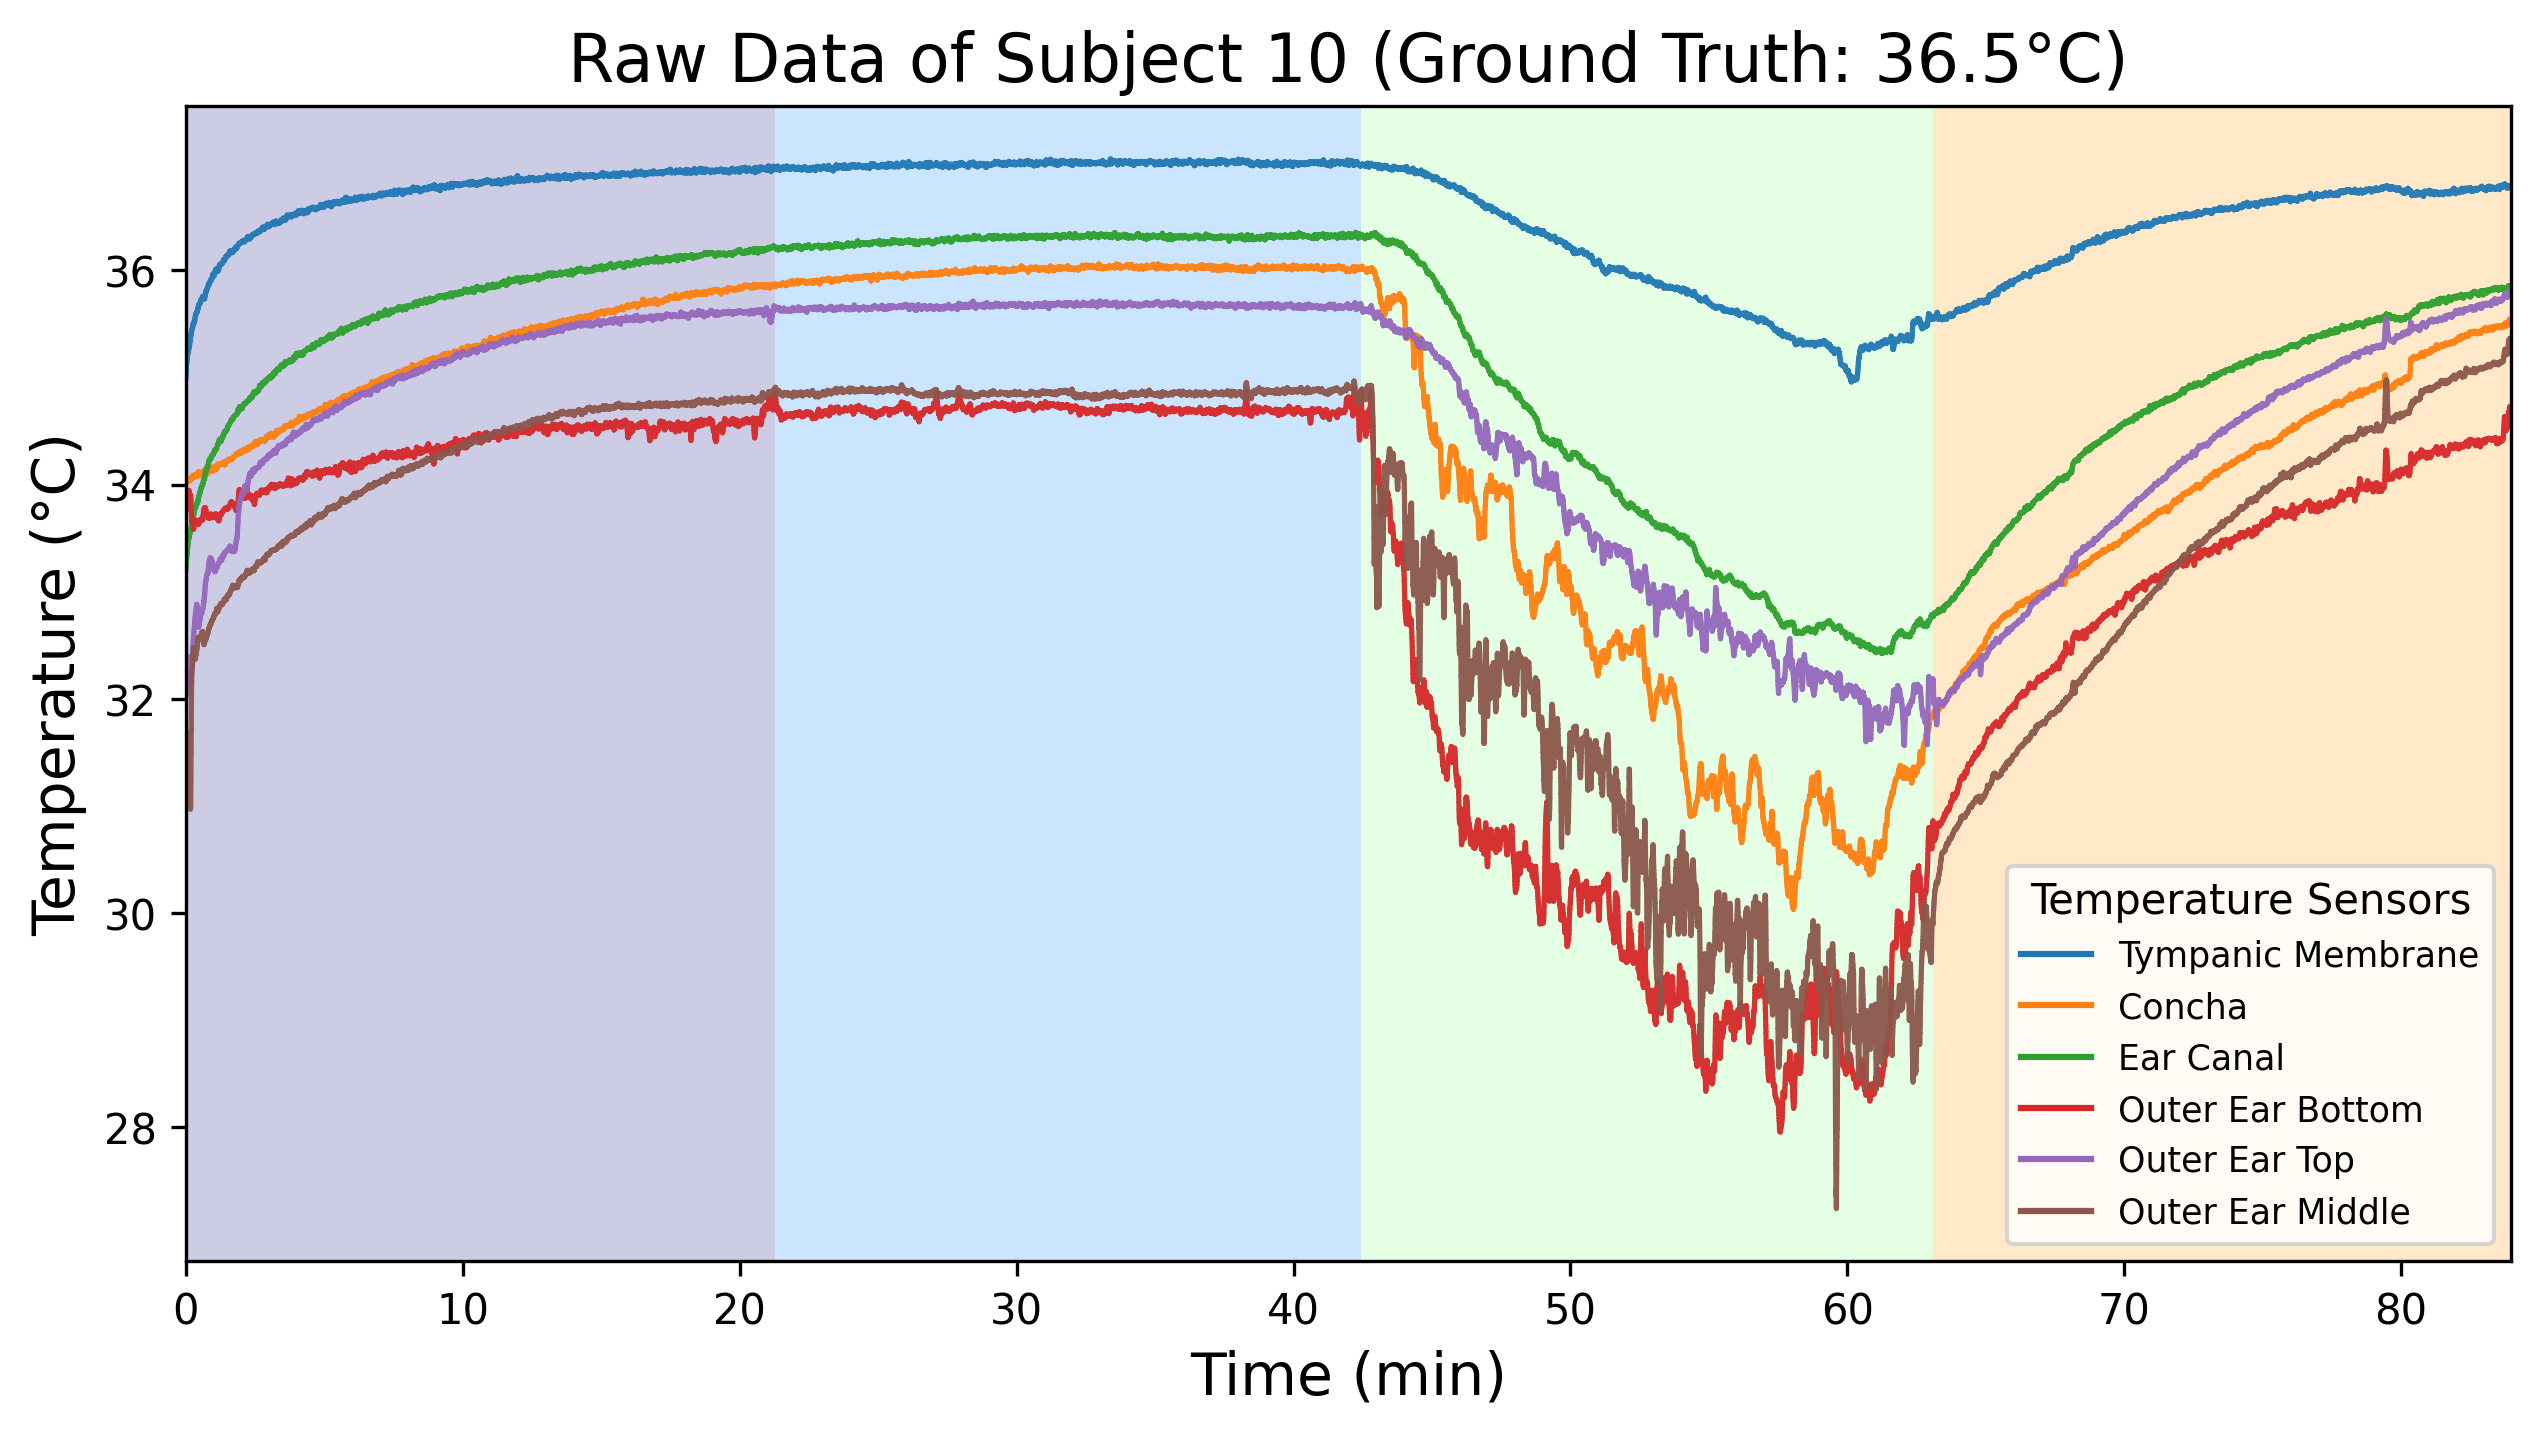
\includegraphics[width=\textwidth]{thesis-doc/images/study1/Logging_person_10_0smoothed_raw_data.png}
    \caption{Raw data of a measurement in study 1 of subject 10. The subject had a body temperature of $36.5^\circ\text{C}$ at the beginning. Phases 1-4 are shown, distinguished by the background color of the plot. In phase 1, the sensor has adjusted and acclimated to the temperature of the subject. After the sensor settled in, Phase 2 measured the temperature while sitting in a room. In phase 3, the subject went for a walk outside. In phase 4, he went back into the room to see how the sensors settled back to the calmer environmental conditions.}
    \label{fig:ch:Evaluation:Study1:RawData}
\end{figure}

\subsection{Hypothesis 1: Lower Temperature Measured on Sensors Behind the Ear}
\label{subsec:Evaluation:Study1:Hypothesis1}

The first hypothesis is to show that a lower temperature is measured behind the ear than in the ear.
For this purpose, the analysis was considered in two perspectives. 
First, only the data points where the subject was sitting were recorded, and second, all data were considered except for the acclimatization phase (phase 1).

In the first perspective, the data were considered at which the subject was seated (phase 2). 
Here, for all subjects, the mean temperature behind the ear was \(36.30^\circ\text{C}\), while the mean temperature inside the ear was \(36.74^\circ\text{C}\). 
To prove a statistically significant difference between the two means, a t-test can be used.
The t-test yielded a p-value of \(0.0424\), which is below the alpha value of \(0.05\).
Since the p-value is below the alpha, this is evidence of a significant difference.
The mean error between the ground truth and the temperature measured behind the ear was \(0.79^\circ\text{C}\), and that for the temperature in the ear was \(0.38^\circ\text{C}\). 
The p-value for the comparison of these errors was \(0.0115\), again indicating a statistically significant difference.
Thus, it is clear that temperature is measured significantly lower behind the ear than in the ear while sitting.

The second perspective now also looks at other phases of the study. 
Now, in addition to the sitting phase (phase 2), the walking phase (phase 3) and the regeneration phase (phase 4) were also considered. 
The mean temperature behind the ear was \(35.33^\circ\text{C}\) and in the ear it was \(36.02^\circ\text{C}\). 
The p-value of the T-test was \(0.0158\), which again is statistically significant.
The mean error behind the ear was \(1.67^\circ\text{C}\) and in the ear it was \(0.98^\circ\text{C}\). 
The p-value for the comparison of these errors was \(0.0158\), which is also statistically significant.

This can also be seen in Figure \ref{fig:eval:study1:hypothesis1_result}.
The two boxplot images show the sitting and walking phases (phase 2 and 3), always zeroed to the temperature measured by the thermometer before the measurement.
During sitting (phase 2), the temperature measured at the tympanic membrane is very close to the temperature measured by the thermometer ($\pm0.25^\circ\text{C}$). 
The sensors in the ear canal and pinna also show high accuracy. 
For the sensors behind the ear, although the median is sometimes very close to the sensors in the ear, the outliers are strongly represented here, which questions the reliability of the signals.
When comparing the sensors behind the ear, the sensor placed at the top behind the ear provides the best results. 
This is due to the position behind the ear, the further below the ear, the more external influences are felt, such as a gust of wind, even if only with slight movements.
This can be seen more clearly in the boxplot for phase 3, while the test subjects were out walking. 
While here also the sensor pointing to the eardrum shows the best results, all other sensors have outliers.
There is also a significant difference between the sensor in the ear canal and the auricle. 
The sensor in the ear canal is further in the ear and thus somewhat more protected from external conditions, which is also evident here. 
The findings of the boxplot from phase 2 are also confirmed for the sensors behind the ear.

The second perspective also confirms the hypothesis that the temperature measured behind the ear is statistically significantly lower than that measured in the ear. 
However, the sensors behind the ear also show a statistically significant higher error compared to the ground truth, especially when the subject is involved in activities such as walking. 
These findings have important implications for the use of ear-based temperature sensors in various applications.

\begin{figure}[!h]
    \centering
    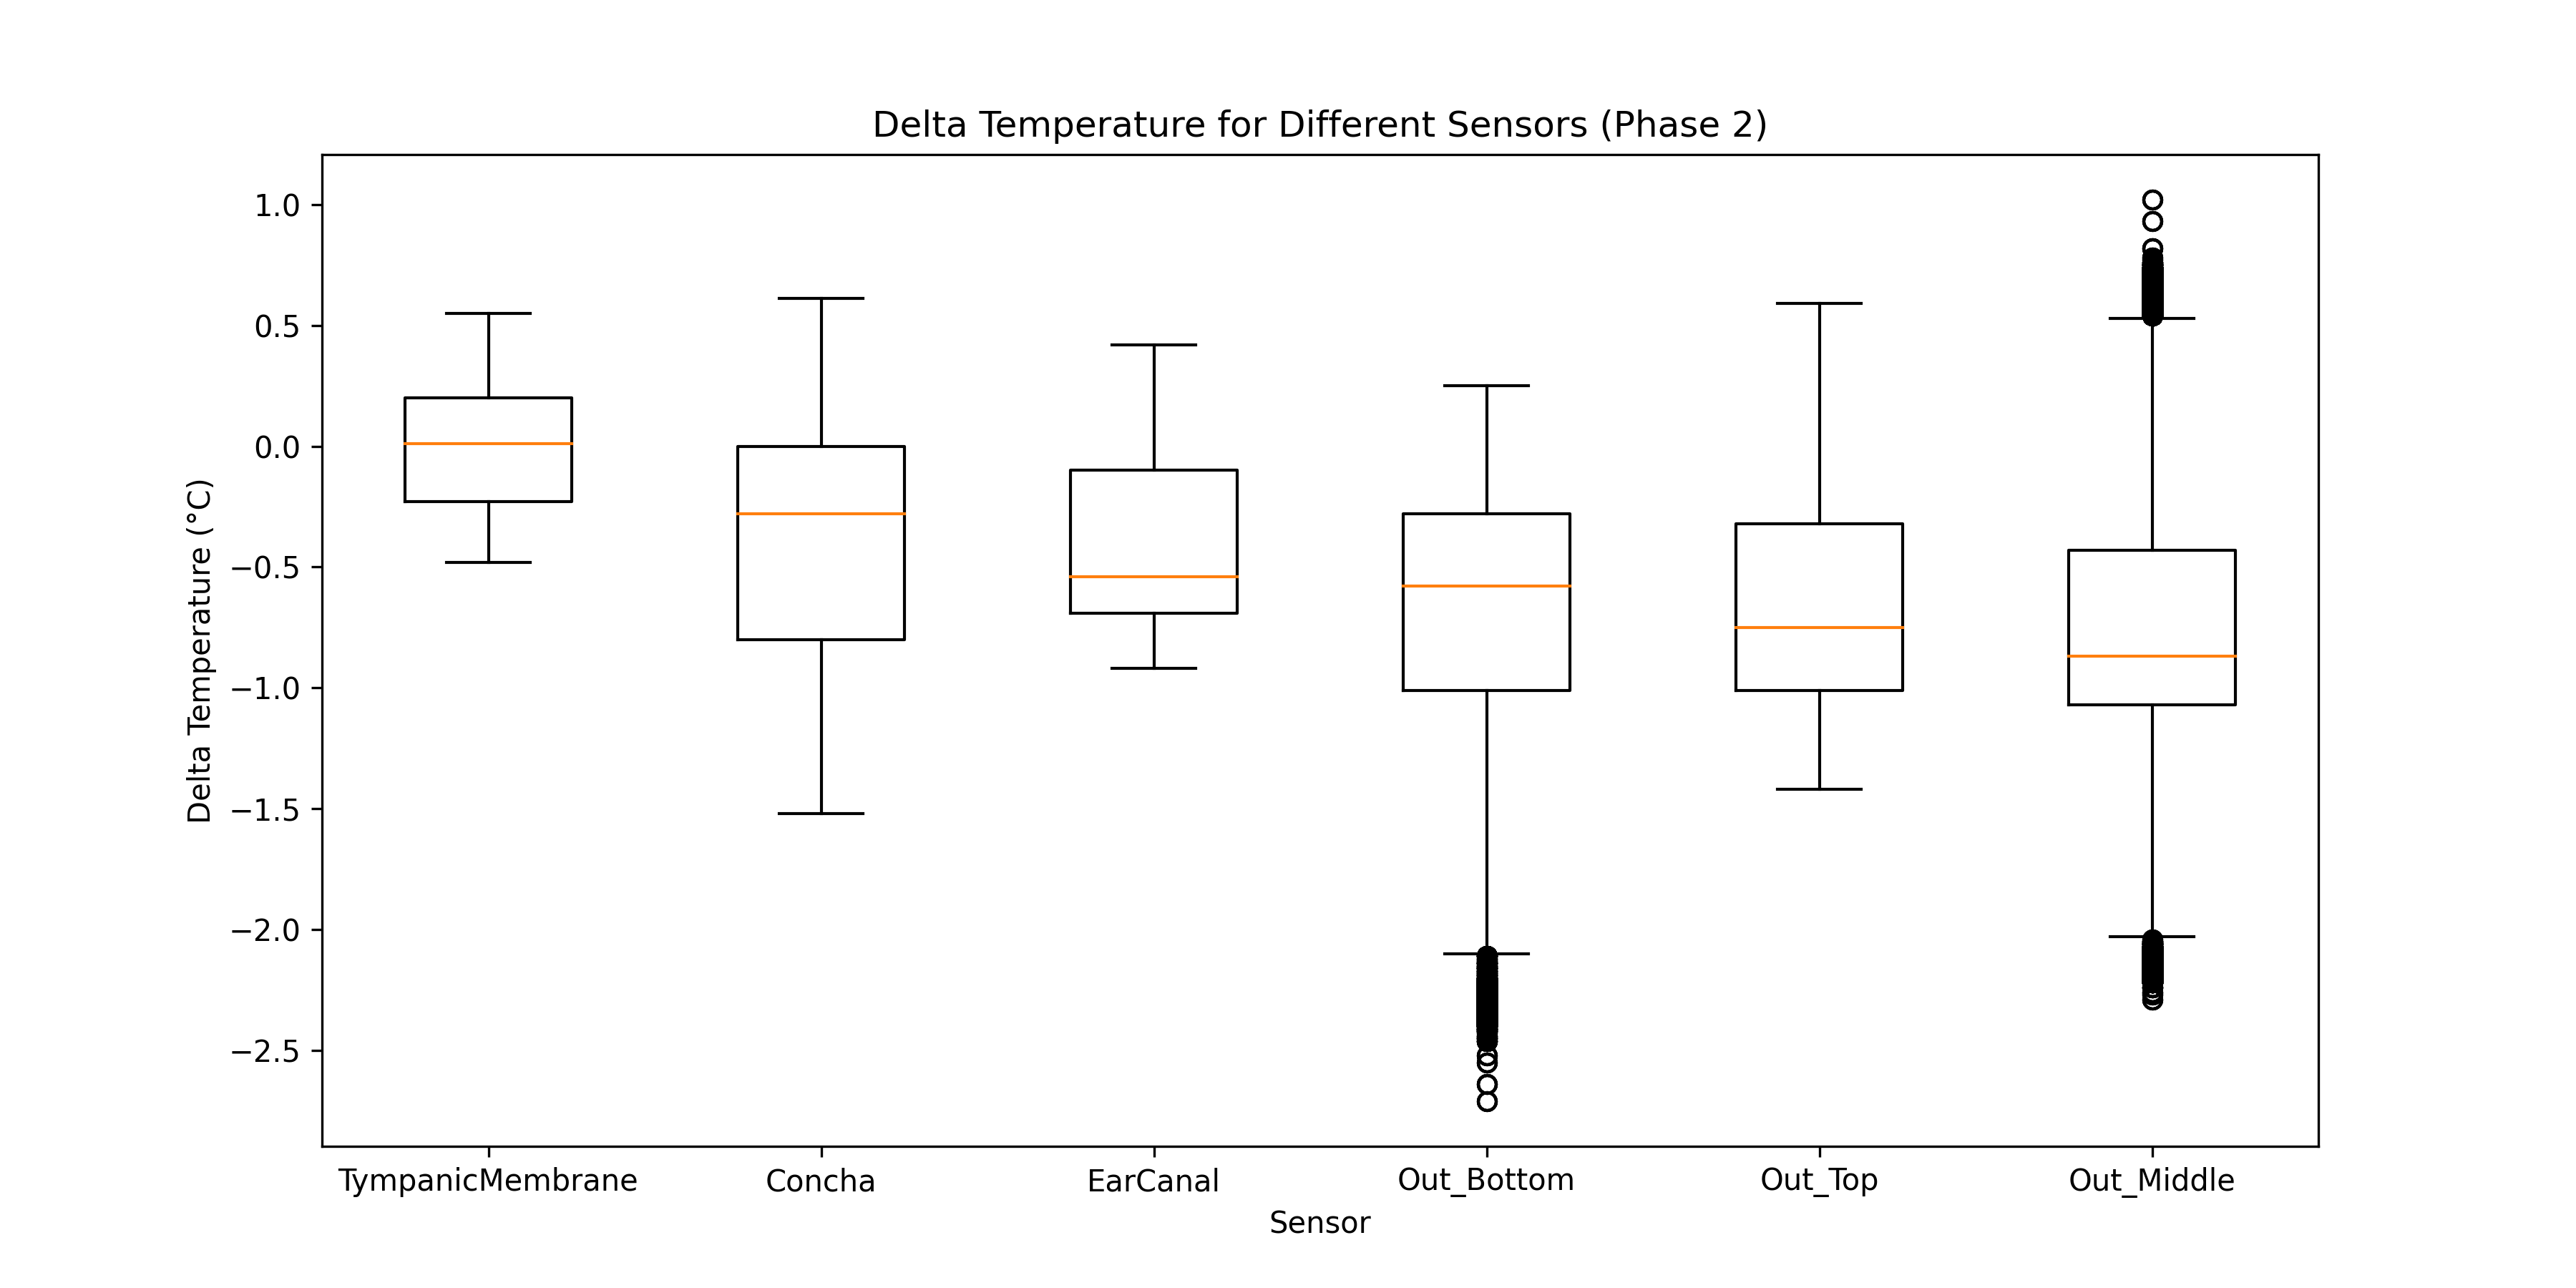
\includegraphics[width=\textwidth]{thesis-doc/images/study1/hypothesis1/hypothesis1_boxplot_phase_2.png}
    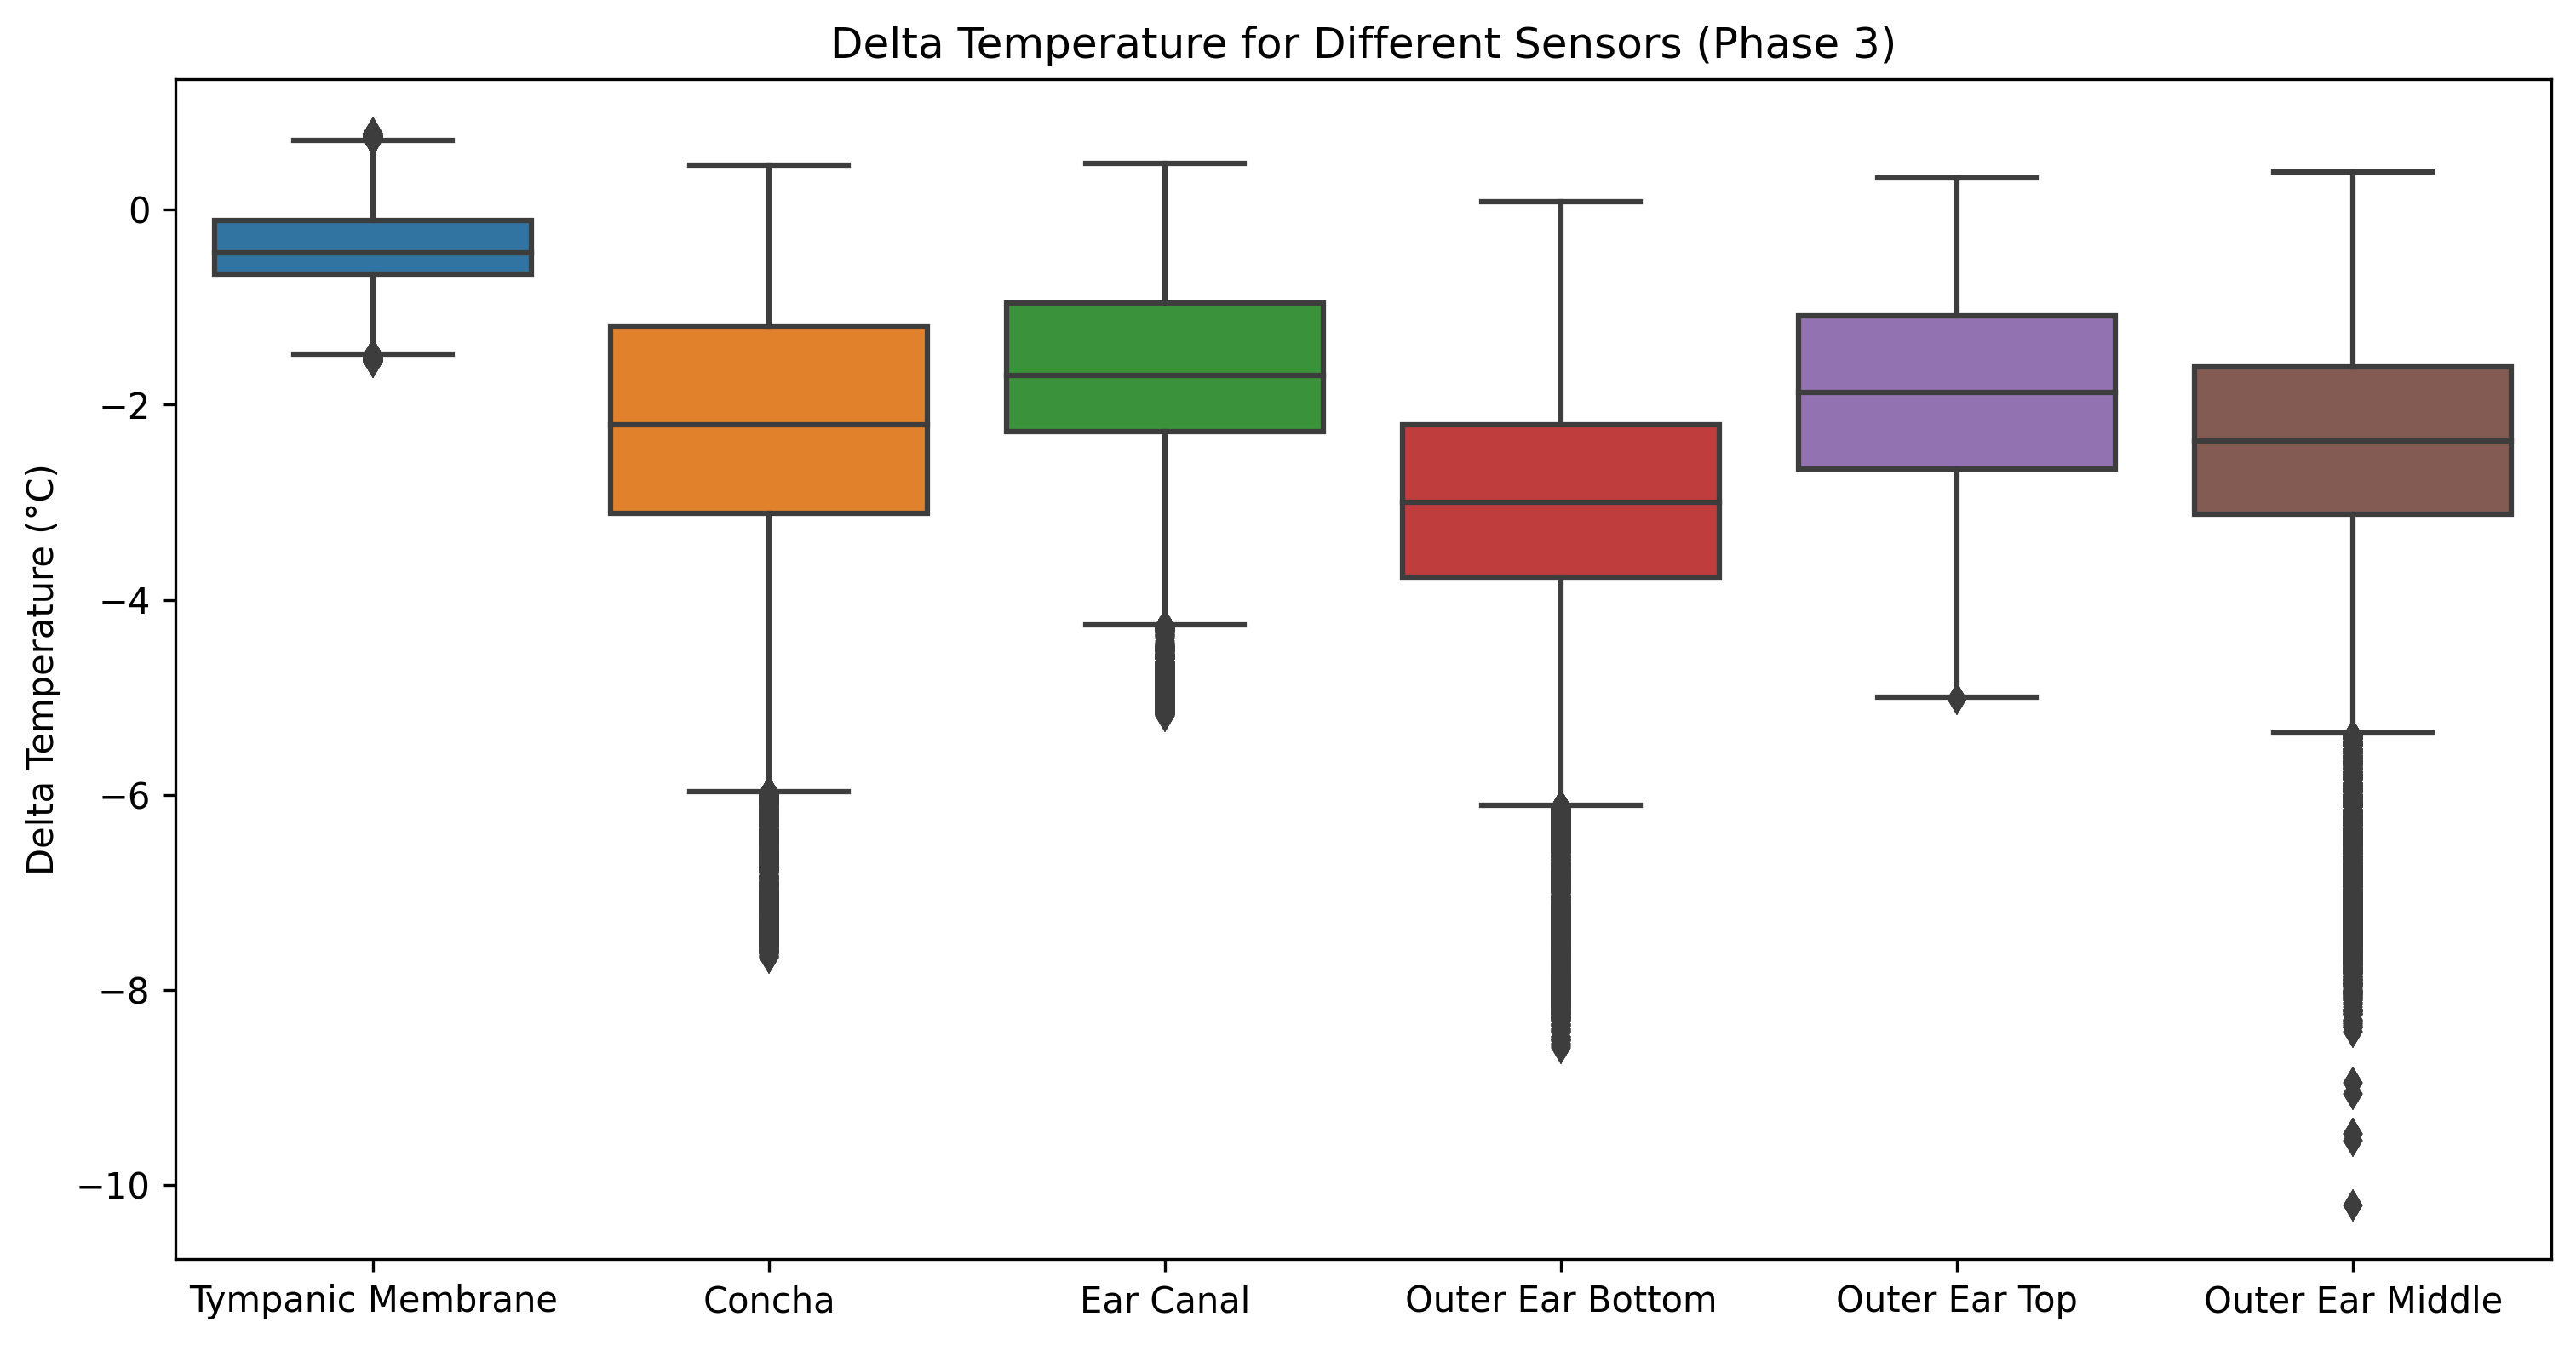
\includegraphics[width=\textwidth]{thesis-doc/images/study1/hypothesis1/hypothesis1_boxplot_phase_3.png}
    \caption{Boxplots visually illustrating the distribution of measured values from different sensor positions during phase 2 (indoor) and phase 3 (outdoor). Central tendencies and their dispersion for the analysis of the sensors under different environments can be seen. Temperature values were subtracted from the thermometer reading to compare all user data together. These visualizations are an essential part of the evaluation of Hypotheses 1 and 2, as they highlight differences in variance and highlight potential outliers.}
    \label{fig:eval:study1:hypothesis1_result}
\end{figure}

\subsection{Hypothesis 2: Variance Difference Indoor/Outdoor}
\label{subsec:Evaluation:Study2:Hypothesis2}

The second hypothesis is to show that the variance in temperature readings from ear-based sensors is lower indoors than outdoors.
This expectation is derived from the fact that the external influences in an indoor environment with closed windows are significantly less than the external influences outside during walking.
To test this hypothesis empirically, the data set of several ear-based temperature sensors at different positions was considered, both indoors and outdoors.
The different situations within the studies were divided into phases. 
Phase 2 represents an indoor measurement, and Phase 3 represents an outdoor measurement during walking.
Here, the temperature values in different areas of the ear were looked at closely.
To prove the hypothesis, the variances per temperature sensor were now calculated for phases 2 and 3 respectively. 
The results show a clear pattern. 
The mean variance for the tympanic sensor $0.00096$ indoors and \(0.107\) outdoors.
This pattern was consistently observed for other sensor locations, such as the auricle with a mean variance of $0.00307$ indoors and $1.134$ outdoors.
A detailed listing of the results can be seen in Table \ref{subsec:Evaluation:Study2:Hypothesis2:mean_variance_table}.
A two-sample T-test was used to statistically compare these variances.
The results provided clear evidence to support the hypothesis.
For example, the p-value for the tympanic sensor was significantly below the Bonferroni-corrected threshold, clearly refuting the null hypothesis.
This pattern is also seen for the other positions in and around the ear, providing extensive empirical support for the hypothesis.
In summary, the data confirm the second hypothesis: temperature measurements with ear-based sensors have significantly lower deviations when taken indoors than outdoors.

\begin{table}[ht]
\centering
\begin{tabular}{|l|c|c|c|c|}
\hline
Sensor & \multicolumn{2}{c|}{Mean Variance} & \multicolumn{2}{c|}{Mean Diff. from} \\
       & \multicolumn{2}{c|}{(in $^\circ\text{C}$)} & \multicolumn{2}{c|}{Ground Truth (in $^\circ\text{C}$)} \\
\hline
 & Indoor & Outdoor & Indoor & Outdoor \\
\hline
TympanicMembrane & 0.00096 & 0.1074 & 0.0071 & -0.6077 \\
Concha & 0.00307 & 1.1339 & -0.3805 & -2.5609 \\
EarCanal & 0.00155 & 0.6456 & -0.3934 & -1.9584 \\
Out\_Bottom & 0.0189 & 1.1098 & -0.7439 & -3.3107 \\
Out\_Top & 0.00694 & 0.6499 & -0.6060 & -2.1198 \\
Out\_Middle & 0.0198 & 1.0982 & -0.7452 & -2.7643 \\
\hline
\end{tabular}
\caption{Mean variance and mean variance of deviation from ground truth for different sensors. Phases 2 (indoor) and 3 (outdoor) were considered. From this, the variances were calculated for each sensor and averaged over all subjects. In addition, the distance to ground truth was displayed to display the value of the accuracy of the variance.}
\label{subsec:Evaluation:Study2:Hypothesis2:mean_variance_table}
\end{table}

\subsection{Hypothesis 3: Relative Changes in Temperature Readings}
\label{subsec:Evaluation:Study1:Hypothesis3}
The third hypothesis examines the correlation between relative changes in temperature readings from different sensor locations at Phases 2 and 3.
This is to understand the constancy between different sensor readings, especially in relation to changing weather conditions.
Pearson's correlation coefficient is used for analysis.
This is a way of determining the linear relationship between two variables and is used as a measure of the strength of the correlation. 
The correlation coefficient takes values between $-1$ and $1$. 
The calculation of the coefficient is performed for phase 2 and 3 per sensor pair. 
The results of all subjects are then averaged and presented in the form of a heat map in Figure \ref{fig:eval:study1:hypothesis3_result}.
It can be seen in Phase 2 that sensors located in a similar anatomical region show similar moderate to strong positive correlations. 
However, between sensors inside the ear and outside the ear, the correlations are generally rather weak to partially negative, suggesting different behavior under the same environmental conditions.
In contrast, phase 3 shows a high degree of positive correlation between all pairs of sensors, often exceeding a coefficient of 0.9.
This high correlation indicates that all sensors exhibit remarkable consistency in their readings. 
However, here the temperature dropped sharply as the users left the room and went for a walk outside. 
The high temperature drop is then reflected in the correlation.
As can be seen in table \ref{subsec:Evaluation:Study2:Hypothesis2:mean_variance_table}, the measured temperature drops by as much as $2.7643^\circ\text{C}$ in some cases.
Due to this, the correlation in this case is not a good example.
More informative here is the mean absolute deviation.

\begin{figure}[!h]
    \centering
    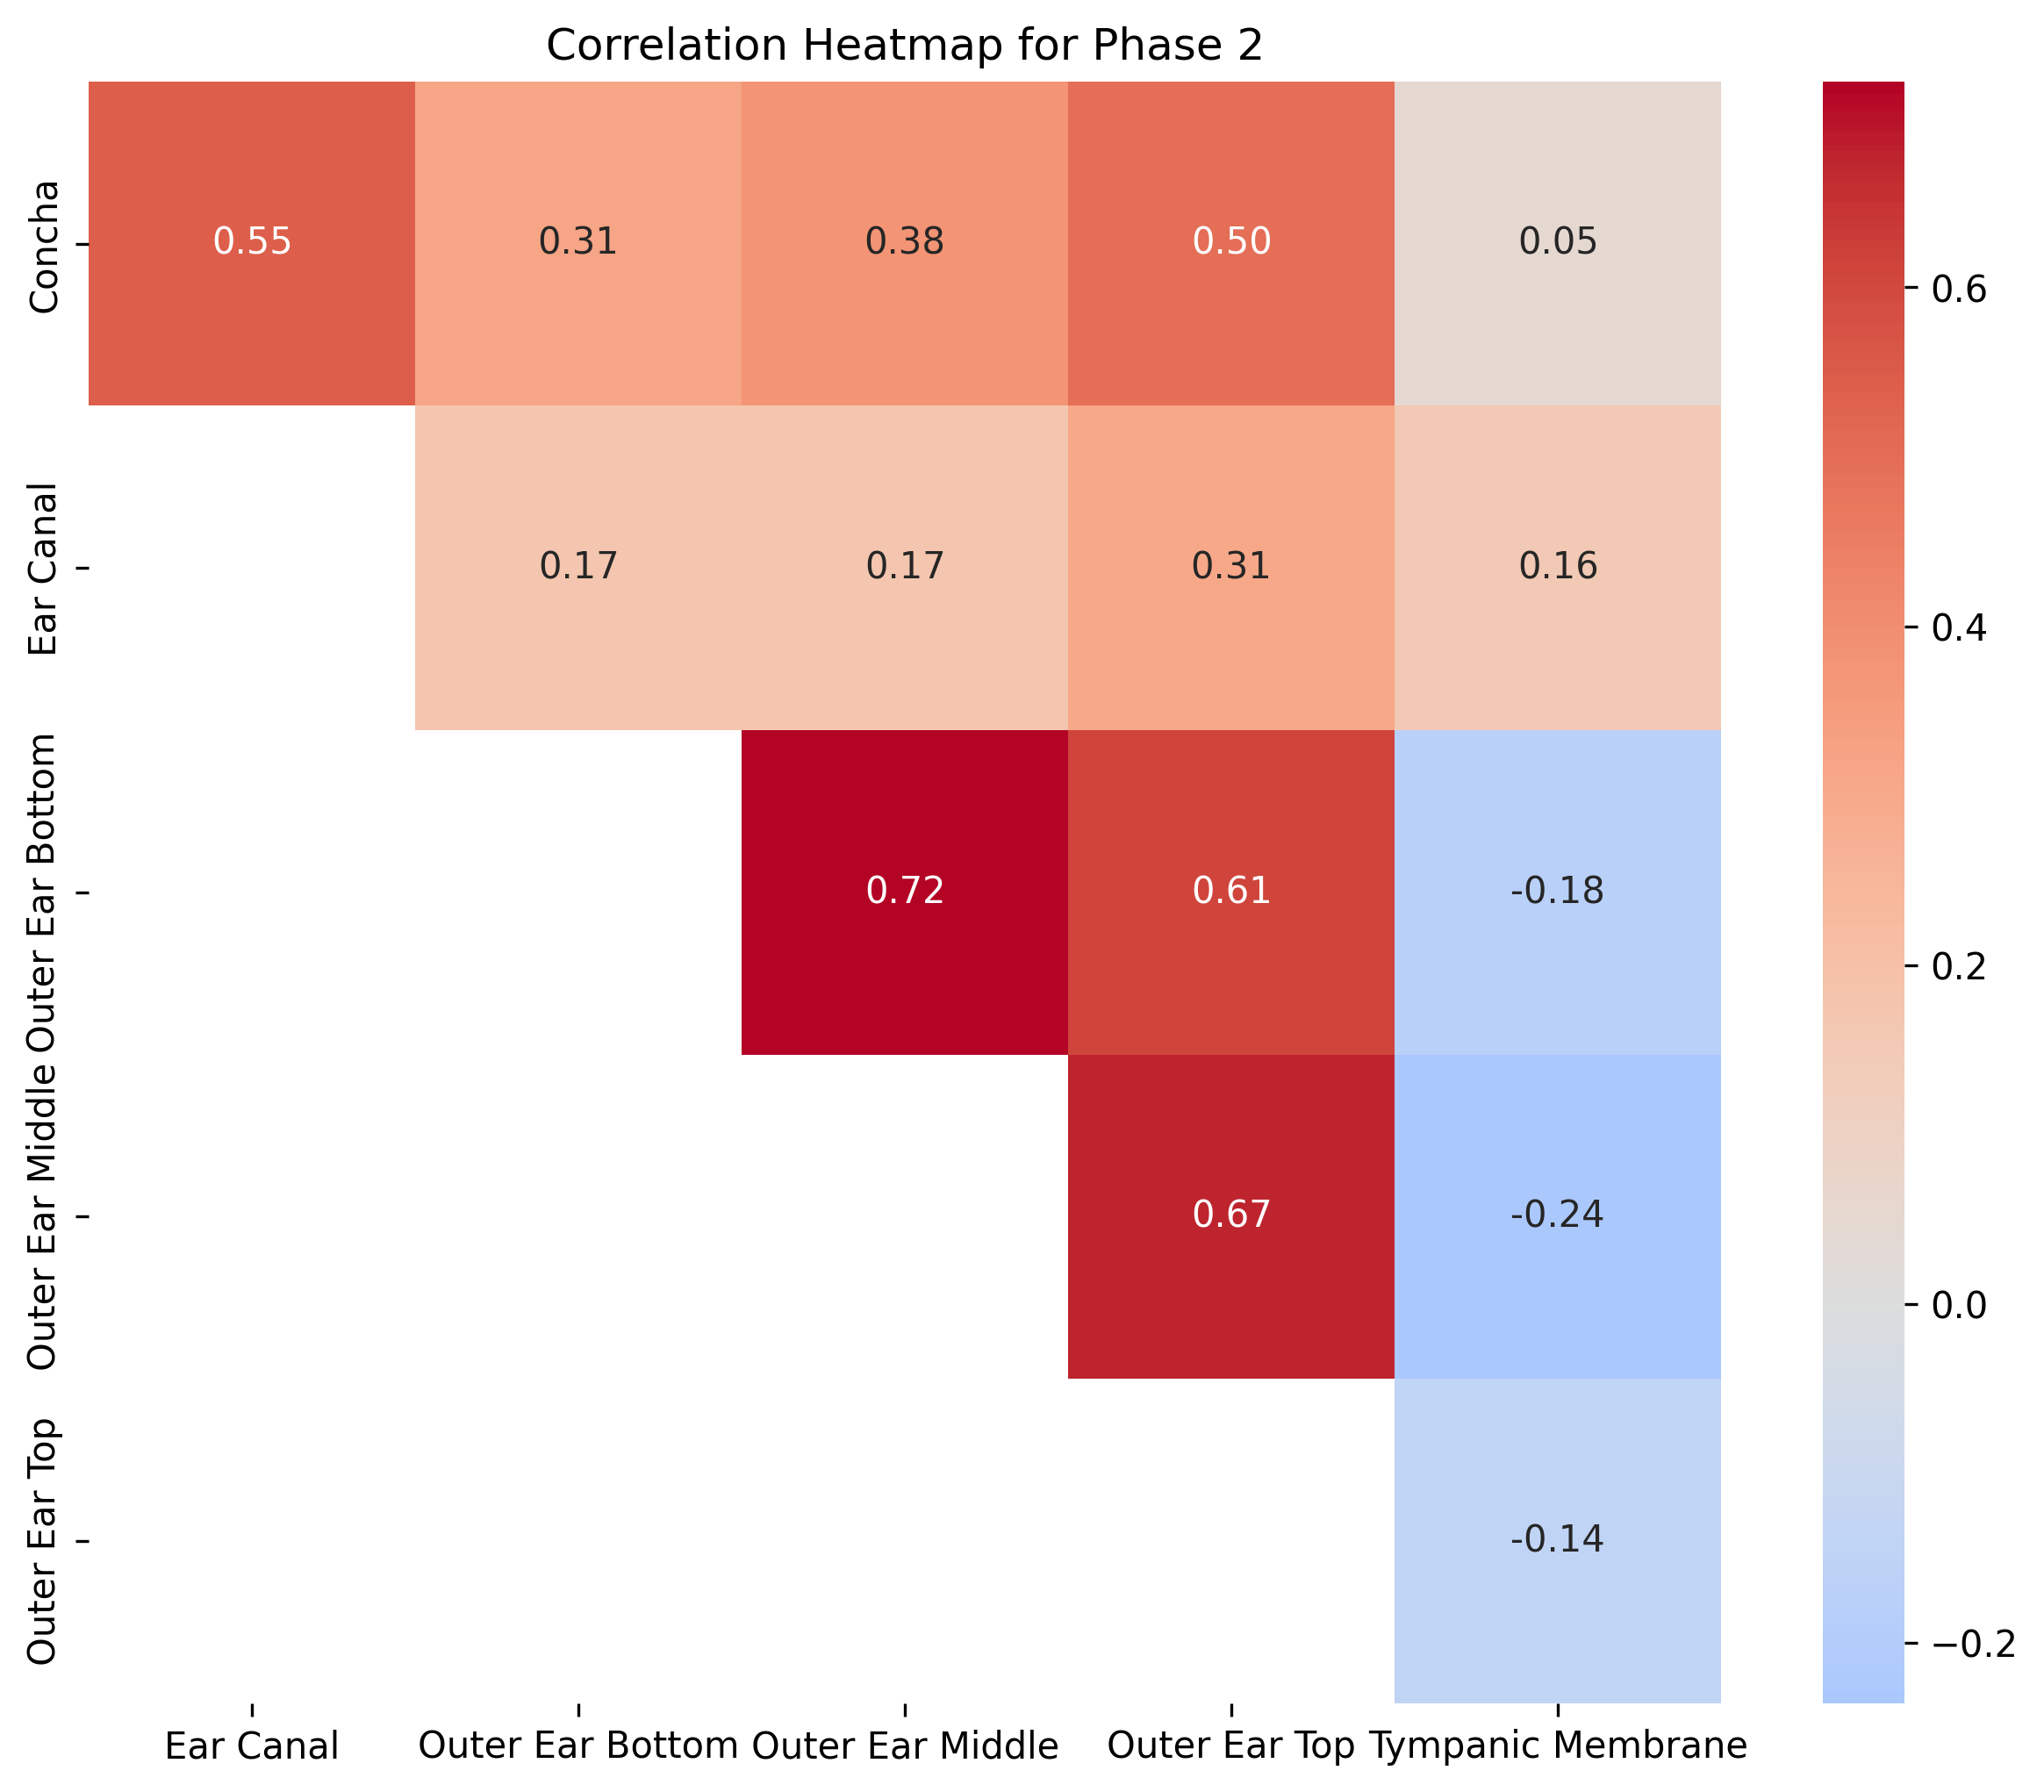
\includegraphics[width=0.9\textwidth]{thesis-doc/images/study1/hypothesis3/Correlation_Heatmap_Phase_2.png}
    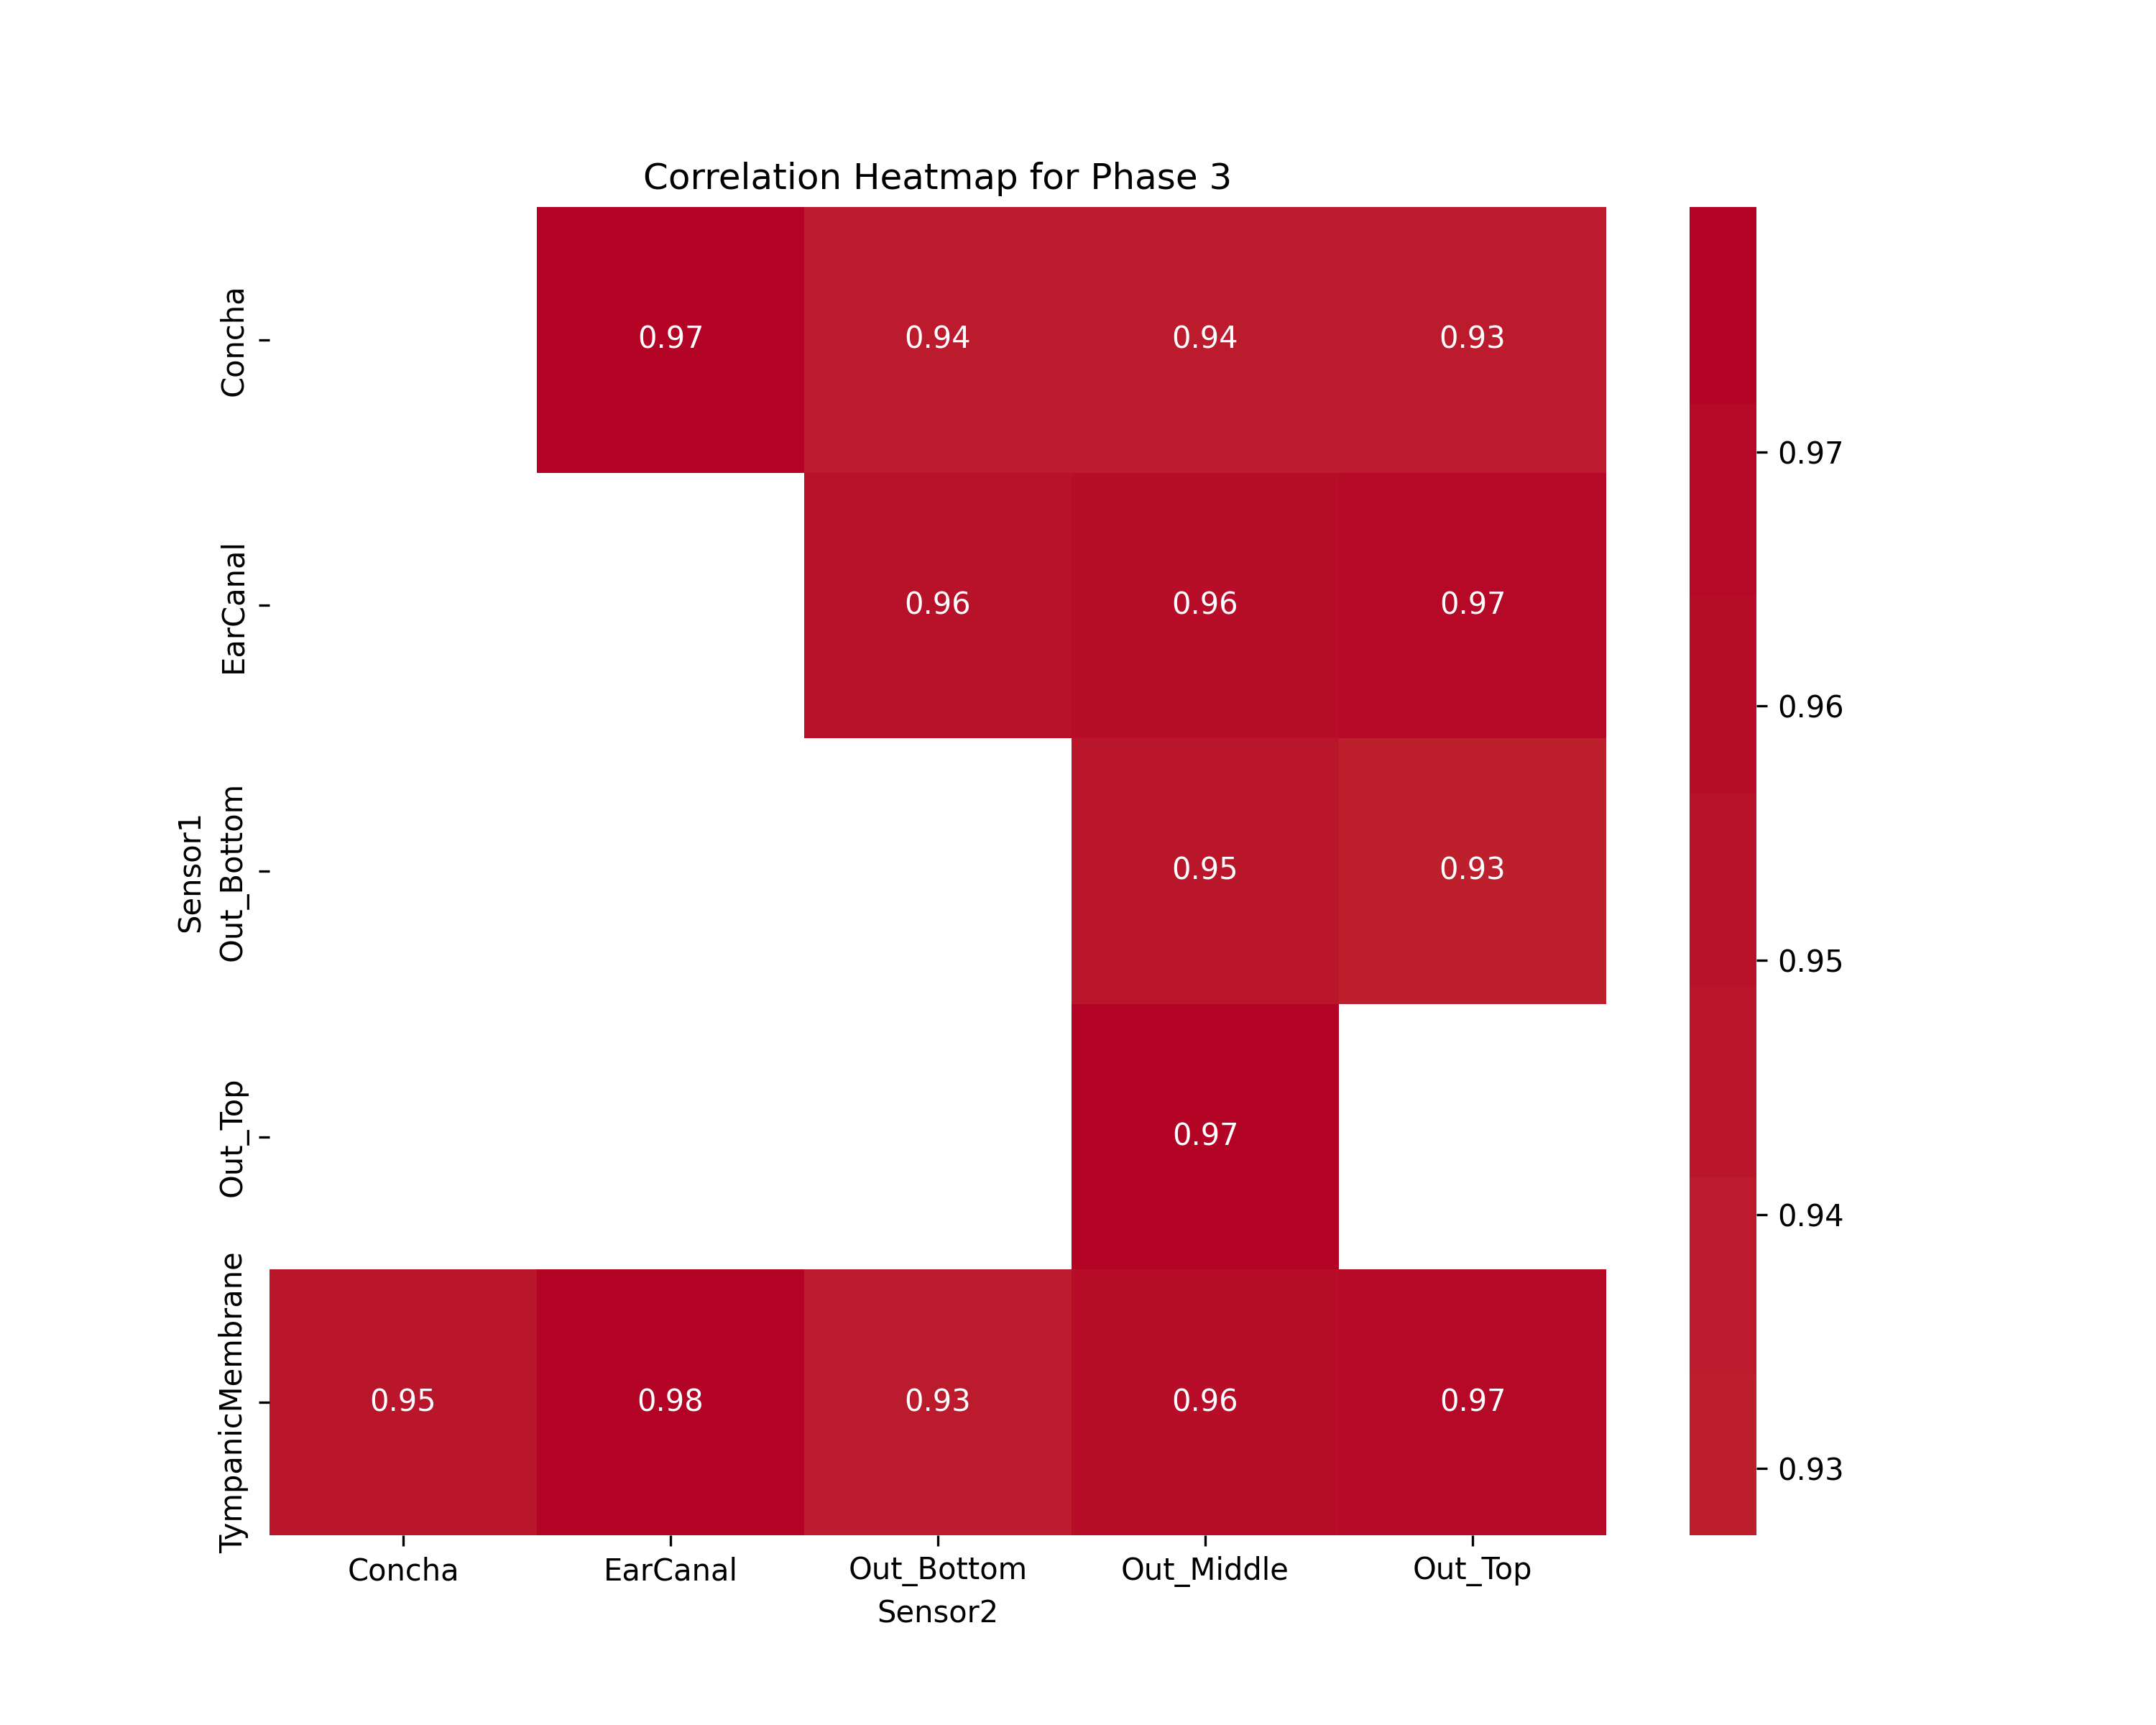
\includegraphics[width=0.9\textwidth]{thesis-doc/images/study1/hypothesis3/Correlation_Heatmap_Phase_3.png}
    \caption{Heat maps showing the correlation matrices of temperature readings from different ear-based sensors during Phase 2 (indoor) and Phase 3 (outdoor). The color-coded matrices provide a visual representation of how strongly each pair of sensors correlates under different conditions. Darker shading represents higher correlation and helps assess consistency between sensor measurements and their sensitivity to environmental changes, providing empirical evidence for Hypothesis 3.}    
    \label{fig:eval:study1:hypothesis3_result}
\end{figure}